\documentclass{standalone}

\usepackage{tikz}
\usetikzlibrary{shapes.geometric}
\begin{document}
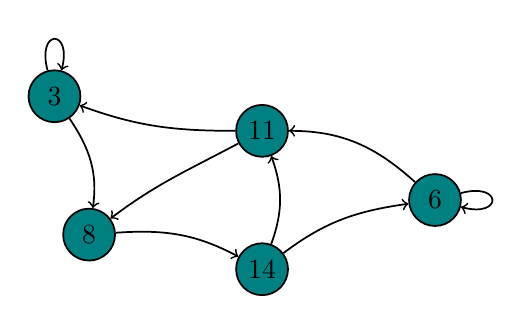
\begin{tikzpicture}
[every node/.style={inner sep=0pt}]
\node (3) [circle, minimum size=18.75pt, fill=teal, line width=0.625pt, draw=black] at (37.5pt, -25.0pt) {\textcolor{black}{3}};
\node (8) [circle, minimum size=18.75pt, fill=teal, line width=0.625pt, draw=black] at (50.0pt, -75.0pt) {\textcolor{black}{8}};
\node (14) [circle, minimum size=18.75pt, fill=teal, line width=0.625pt, draw=black] at (112.5pt, -87.5pt) {\textcolor{black}{14}};
\node (6) [circle, minimum size=18.75pt, fill=teal, line width=0.625pt, draw=black] at (175.0pt, -62.5pt) {\textcolor{black}{6}};
\node (11) [circle, minimum size=18.75pt, fill=teal, line width=0.625pt, draw=black] at (112.5pt, -37.5pt) {\textcolor{black}{11}};
\draw [line width=0.625, ->, color=black, loop above] (3) to (3);
\draw [line width=0.625, ->, color=black, loop right] (6) to (6);
\draw [line width=0.625, ->, color=black] (11) to  [in=340, out=180] (3);
\draw [line width=0.625, ->, color=black] (3) to  [in=82, out=304] (8);
\draw [line width=0.625, ->, color=black] (8) to  [in=152, out=4] (14);
\draw [line width=0.625, ->, color=black] (14) to  [in=188, out=37] (6);
\draw [line width=0.625, ->, color=black] (14) to  [in=290, out=70] (11);
\draw [line width=0.625, ->, color=black] (11) to  [in=37, out=208] (8);
\draw [line width=0.625, ->, color=black] (6) to  [in=0, out=138] (11);
\end{tikzpicture}
\end{document}
